\documentclass[10pt, a4paper]{article}
\usepackage[utf8]{inputenc}
\usepackage[spanish]{babel}

\usepackage{varwidth}
\usepackage{graphicx}
\usepackage{eurosym} % para el euro

\usepackage[T1]{fontenc} % Use 8-bit encoding that has 256 glyphs


\usepackage[hmarginratio=1:1,top=32mm,columnsep=20pt]{geometry} % Document margins
\usepackage[hang, small,labelfont=bf,up,textfont=it,up]{caption} % Custom captions under/above floats in tables or figures

\usepackage{float} % Required for tables and figures in the multi-column environment - they need to be placed in specific locations with the [H] (e.g. \begin{table}[H])

\usepackage{hyperref} % For hyperlinks in the PDF


\usepackage{amsmath,amssymb}


\usepackage{titlesec} % Allows customization of titles
\renewcommand\thesection{} % Roman numerals for the sections
\renewcommand\thesubsection{\alph{subsection}} % Roman numerals for subsections
\titleformat{\section}[block]{\large\scshape\centering}{\thesection}{1em}{} % Change the look of the section titles
\titleformat{\subsection}[block]{\large}{\thesubsection.}{1em}{} % Change the look of the section titles

\usepackage{fancyhdr} % Headers and footers
\pagestyle{fancy} % All pages have headers and footers
\fancyhead{} % Blank out the default header
\fancyfoot{} % Blank out the default footer
\fancyhead[C]{Sergio García Prado $\bullet$ Mayo 2016 $\bullet$ Modelos para la Toma de Decisiones $\bullet$ Tarea 2} % Custom header text
\fancyfoot[RO,LE]{\thepage} % Custom footer text

%----------------------------------------------------------------------------------------
%	TITLE SECTION
%----------------------------------------------------------------------------------------

\title{\vspace{-15mm}\fontsize{24pt}{10pt}\selectfont\textbf{Modelos para la Toma de Decisiones: Tarea 2}} % Article title

\author{
\large
\textsc{Sergio García Prado}\\[2mm] % Your name
\normalsize Universidad de Valladolid \\ % Your institution
\vspace{-5mm}
}
\date{}

%----------------------------------------------------------------------------------------

\begin{document}

	\maketitle % Insert title

	\thispagestyle{fancy} % All pages have headers and footers

%----------------------------------------------------------------------------------------
%	TEXT
%----------------------------------------------------------------------------------------

    \section{Ejercicio 1}

        \begin{figure}[H]
        \centering
            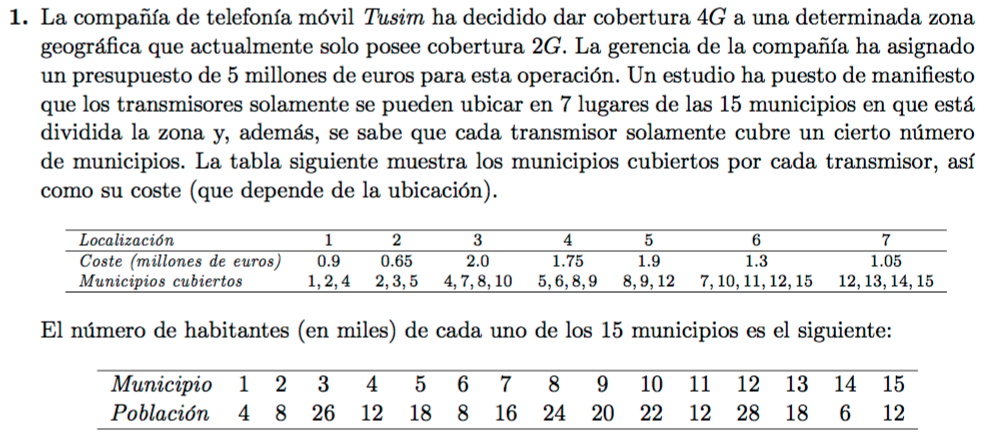
\includegraphics[width=\textwidth]{res/exercise-1.png}
        \end{figure}


		\subsection{Formular un modelo de PLE para determinar dónde se deben construir los transmisores para cubrir la mayor población con el límite del presupuesto de 5 millones de euros.}

			\paragraph{}
			Inicialmente puede pareceder que para modelar el problema harían falta más variables de las necesarias para resolver el problema, ya que intuitivamente necesitaríamos 7 variables para representar si se construye o no un transmisor y otras 15 para determinar si se cubre un municipio o no, es decir, en total necesitaríamos 22 variables. Pero si nos fijamos bien descubrimos que algunas de las poblaciones solo se pueden cubrir por un único transmisor por lo que son equivalentes. Modelando el problema de esta manera llegamos a la conclusión de que son necesarias $9 + 7 = 16$ variables, por lo que nos hemos ahorrado 6 variables y 6 restricciones.

			\paragraph{}
			La modelización del problema como de PLE es la siguiente:

			\begin{itemize}
				\item \(x_{i} = \) Se construye un transmisor en la localización i. $1<= i <= 7$

				\item \(p_{j} \) La población j tiene señal de comunicación. $j \in {2,4,5,7,8,9,10,12,15}$ Nota: no es  $1<= j <= 15$ por las razones expuestas en el parrafo anterior.
			\end{itemize}

			\[
				\begin{split}
					\text{Max} z = 4x_{1} + 8p_{2} + 26x_{2} + 12p_{4} +18p_{5} + 8x_{4} + 16p_{7} \\
						+ 24p_{8} +20p_{9} + 22p_{10}  +  12x_{6} + 28p_{12} + (18+6)x_{7} + 12p_{15} \\ \\
						0.9x_1 + 0.65x_2 + 2x_3 + 1.75x_4 + 1.9x_5 + 1.3x_6 + 1.05 x_7 <= 5 \\ \\
						p_2 <= x_1 + x_2\\ \\
						p_4 <= x_1 + x_3\\ \\
						p_5 <= x_2 + x_4\\ \\
						p_7 <= x_3 + x_6\\ \\
						p_8 <= x_3 + x_4 + x_5\\ \\
						p_9 <= x_4 + x_5\\ \\
						p_{10} <= x_3 + x_6\\ \\
						p_{12} <= x_5 + x_6 + x_7\\ \\
						p_{15} <= x_6 + x_7\\ \\
						p_{j}, x_{i} \in {0,1}\\ \\
				\end{split}
			\]


		\subsection{?`Cuántos transmisores se deben construir y en qué lugares? ?`Cuál es el tamaño de la población cubierto por esos transmisores? ?`Y el coste de la operación? ?`Existen municipios sin cubrir por esos transmisores?. Justificar las respuestas.}

			\paragraph{}



	\section{Ejercicio 2}

        \begin{figure}[H]
        \centering
            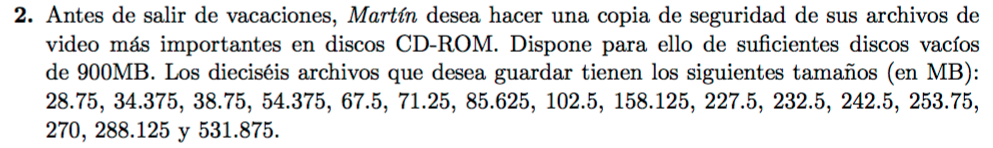
\includegraphics[width=\textwidth]{res/exercise-2.png}
        \end{figure}


		\subsection{Suponiendo que Martín no tiene ningún programa para comprimir los archivos, formular un modelo de PLE para determinar cómo se deben distribuir los archivos con el fin de reducir al mínimo el número de discos CD-ROM que debe utilizar.}

			\paragraph{}
			Modelizaremos el problema como si se pudiera dar el peor caso, es decir, que cada fichero tan solo entrase en un CD-ROM. A pesar de ello para resolverlo hemos ido probando primero con 1 CD-ROM, pero al ver que no era factible seguidamente probamos con 2 y así sucesivamente hasta que hemos encontrado la solución óptima (3 CD-ROM's). El movivo de que sea así es que sino para resolver el problema necesitariamos $16 x 16 = 256$ variables de las cuales la mayoría serían innecesarias.

			\begin{itemize}

				\item \(x_{ij} => \) Variable binaria que indica si se en el CD-ROM i se alojará el fichero j.  $i \in \{1,...,16\}$, $j \in \{1,...,16\}$

				\item \(c_{i} => \) Variables que indica si se utilizará el CD-ROM i.
			\end{itemize}
			\[
				\begin{split}
					\text{Min} z = \sum_{i=1}^{16} c_{i} \\ \\
						0.9x_{i1} + 0.65x_{i2} + 2x_{i3} + 1.75x_{i4} \\
						+ 1.9x_{i5} + 1.3x_{i6} + 1.05 x_{i7} + 1.05 x_{i8} \\
						+ 0.65x_{i9} + 2x_{i10} + 1.75x_{i11}  + 1.75x_{i12}\\
						+ 1.9x_{i13} + 1.3x_{i14} + 1.05 x_{i15} + 1.05 x_{i16} <= 900c_{i}, i \in \{1,...,16\}\\ \\
					 	\sum_{i=1}^{16} x_{ij} = 1, j \in \{1,...,16\}\\ \\
						c_{i}, x_{ij} \in {0,1}, i \in \{1,...,16\},j \in \{1,...,16\}\\ \\
				\end{split}
			\]
		\subsection{?`Cuántos CD debe utilizar y qué archivos debe ubicar en cada uno de ellos? Justificar la respuesta.}




	\section{Ejercicio 3}

        \begin{figure}[H]
        \centering
            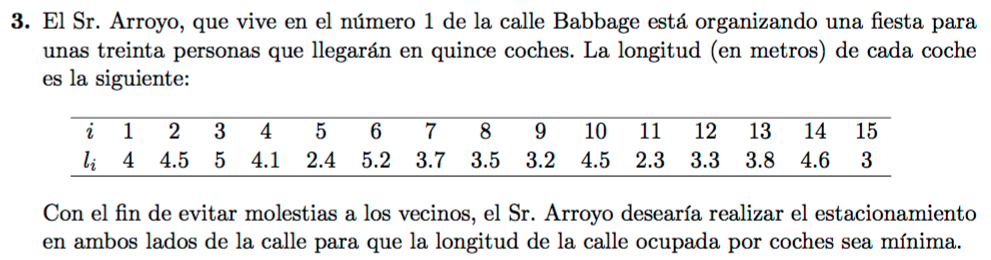
\includegraphics[width=\textwidth]{res/exercise-3.png}
        \end{figure}


		\subsection{Formular un modelo PLE para resolver el problema.}

			\paragraph{}
			Para modelar este problema tenemos que descomponer el valor absoluto de la diferencia entre la longitud que ocupan los coches aparcados a un lado de la calle y los del otro dado que es el valor que queremos minimizar. Añadimos dos variables auxiliares que contendrán la longitud de cada uno de los lados para facilitar la lectura de los resultados.

			\paragraph{}
			Por lo tanto modelizaremos el problema de la siguiente manera:

			\begin{itemize}
				\item \(c_{i} => \) Longitud en metros del lado i de la calle. $i \in \{1,2\}$

				\item \(x_{ij} => \) Variable binaria que indica si se aparca en el lado i de la calle el coche j  $i \in \{1,2\}$, $j \in \{1,...,15\}$,

				\item \(y^{+}, y^{-} => \) Variables que descomponen la parte positiva y negativa de la diferencia entre un lado y otro de la calle.
			\end{itemize}

			\[
				\begin{split}
					\text{min} z = y^{+} + y^{-} \\ \\
						y^{+} - y^{-} = c_1 - c_2 \\ \\
						c_i = 4x_{i1} + 4.5x_{i2} + 5x_{i3} + 4.1x_{i4} + 2.4x_{i5} + 5.2x_{i6} + 3.7x_{i7} + 3.5x_{i8} \\
						+ 3.2x_{i9} + 4.5x_{i10} + 2.3x_{i11} + 3.3x_{i12} + 3.8x_{i13} + 4.6x_{i14} + 3x_{i15}, i \in \{1,2\}\\ \\
						x_{1j} + x_{2j} = 1, j \in \{1,...,15\} \\ \\
						x_{ij} \in \{0,1\}, i \in \{1,2\},j \in \{1,...,15\} \\ \\
						c_{i}, y^{+}, y^{-} >= 0, i \in \{1,2\}\\ \\
				\end{split}
			\]
		\subsection{Indicar la solución óptima del modelo planteado en el apartado anterior.}

			\paragraph{}


		\subsection{Supongamos ahora que en uno de los lados de la calle no deben ocupar más de 15 metros. Formular y resolver este nuevo problema.}

			\paragraph{}
			Para resolver este nuevo problema tendremos que definir una nueva variable binaria que denominaremos \textbf{b} y utilizaremos para representar la dicotomía entre cual de los dos lados de la calle es el que no podrá superar los 15 metros. A este nuevo problema habrá que añadirle dos restricciones correspondientes a la dicotomía. Por lo tanto la modelización es la siguiente:

			\[
				\begin{split}
					\text{min} z = y^{+} + y^{-} \\ \\
						y^{+} - y^{-} = c_1 - c_2 \\ \\
						c_1 - 15 <= Mb \\ \\
						c_2 - 15 <= M(1-b) \\ \\
						c_i = 4x_{i1} + 4.5x_{i2} + 5x_{i3} + 4.1x_{i4} + 2.4x_{i5} + 5.2x_{i6} + 3.7x_{i7} + 3.5x_{i8} \\
						+ 3.2x_{i9} + 4.5x_{i10} + 2.3x_{i11} + 3.3x_{i12} + 3.8x_{i13} + 4.6x_{i14} + 3x_{i15}, i \in \{1,2\}\\ \\
						x_{1j} + x_{2j} = 1, j \in \{1,...,15\} \\ \\
						x_{ij} \in \{0,1\}, i \in \{1,2\},j \in \{1,...,15\} \\ \\
						b, c_{i}, y^{+}, y^{-} >= 0, i \in \{1,2\}\\ \\
				\end{split}
			\]




	\section{Resultados WinQSB}

		\begin{figure}[H]
		\centering
			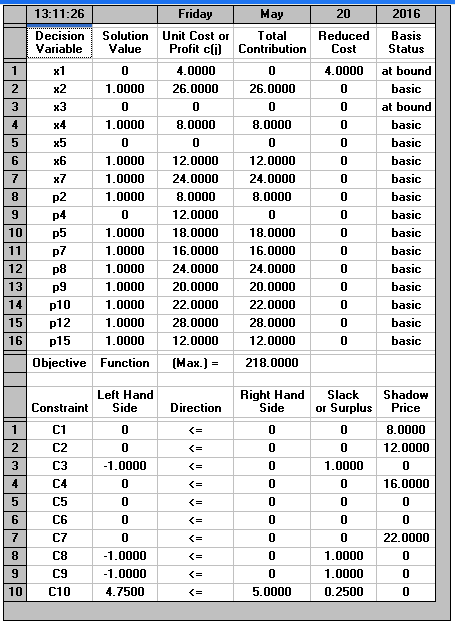
\includegraphics[width=0.75\textwidth]{res/exercise-1-result.png}
		\end{figure}

		\begin{figure}[H]
		\centering
			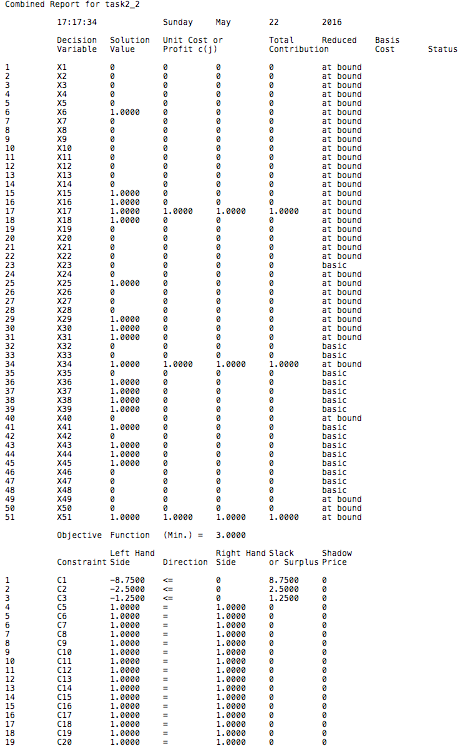
\includegraphics[width=0.75\textwidth]{res/exercise-2-result.png}
		\end{figure}

		\begin{figure}[H]
		\centering
			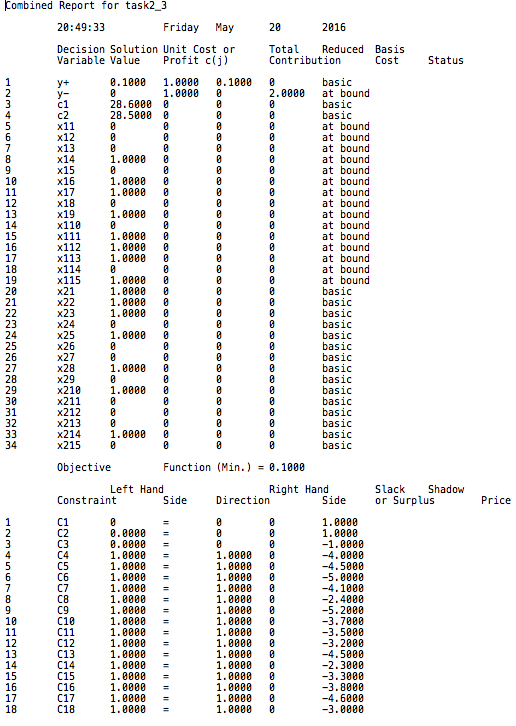
\includegraphics[width=0.75\textwidth]{res/exercise-3-result.png}
		\end{figure}

		\begin{figure}[H]
		\centering
			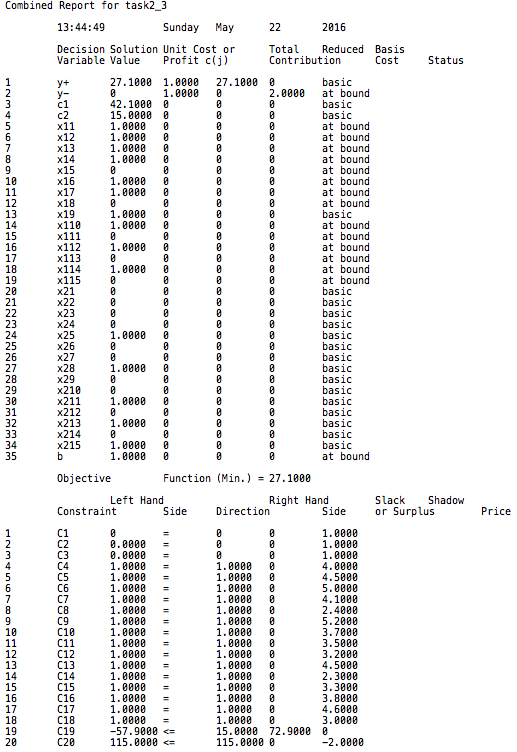
\includegraphics[width=0.75\textwidth]{res/exercise-3-c-result.png}
		\end{figure}
\end{document}
